\documentclass[]{article}

\usepackage{amsmath,amssymb,amsfonts,amsthm}    % Typical maths resource packages
\usepackage{graphicx}                           % Packages to allow inclusion of graphics
\usepackage{hyperref}                           % For creating hyperlinks in cross references
\usepackage[authoryear]{natbib}                 % literature reference style
\usepackage[bf]{caption}
\usepackage{float}
\usepackage{subfig}






% -------------------------------
% --- some layout definitions ---
% -------------------------------

% define topline
\usepackage[automark]{scrpage2}
\pagestyle{scrheadings}
\automark{section}
\clearscrheadings
\ohead{\headmark}

% define citation style
\bibliographystyle{ecta}

% define page size, margin size
\setlength{\headheight}{1.1\baselineskip}
\voffset=-2cm
\hoffset=-3cm
\textheight24cm
\textwidth15.5cm
\topmargin1cm
\oddsidemargin3cm
\evensidemargin3cm

% define line line spacing = 1.5
\renewcommand{\baselinestretch}{1.5}

% define second level for `itemizing'
\renewcommand{\labelitemii}{-}




% --------------------------------------
% --------------------------------------
% --------------------------------------
% --- the structure the tex document ---
% ---  (this our recommendation) -------
% frontmatter:
%   - titlepage (mandatory),
%   - acknowledgement,
%   - abstract,
%   - table of contents (mandatory),
%   - list of abbreviations (not mandatory),
%   - list of figures (not mandatory),
%   - list of tables  (not mandatory) .
%
% body of the thesis (the structure of the thesis body is not mandatory, but the list of literature is mandatory):
%   - introduction,
%   - methods,
%   - data,
%   - results,
%   - conclusion,
%   - literature (mandatory),
%   - appendix (figures, tables).
%
% last page:
%   - declaration of authorship (mandatory).
% --------------------------------------
% --------------------------------------
% --------------------------------------

\begin{document}

% -------------------------------
% --- frontmatter: Title page ---
% -------------------------------

\thispagestyle{empty}
\begin{center}

    {\Large{\bf Bachelor's/Master's Thesis Title}} \vspace{0.5cm}


    {\normalsize Bachelor's/Master's Thesis submitted\\\vspace{0.5cm}
    to}\\\vspace{0.5cm}
    {\normalsize{\bf Prof. Dr. Petra Burdejova}} \\\vspace{0.5cm}
    {\normalsize{\bf Prof. Dr. Awdesch Melzer}} \\\vspace{0.5cm}
    {\normalsize Humboldt-Universit\"at zu Berlin \\
    School of Business and Economics \\
    Institute for Statistics and Econometrics \\
    Chair of Econometrics} \vspace{1cm}


    {\normalsize by \\\vspace{0.5cm}
     Sahnoune Ammar
    (591358)} \vspace{1cm}


    {\normalsize in partial fulfillment of the requirements \\
    for the degree of \\
    {\bf Master of Statistic} \\
    Berlin, August 12, 2018}

\end{center}




% -----------------------------
% --- frontmatter: Abstract ---
% -----------------------------
\newpage
\pagestyle{plain}
\pagenumbering{roman}   % define page number in roman style
\setcounter{page}{1}    % start page numbering


                      






% -----------------------------
% --- frontmatter: Contents ---
% -----------------------------
\newpage
\tableofcontents
\clearpage



% -------------------------------
% --- main body of the thesis ---
% -------------------------------
\newpage
\pagestyle{plain}
\setcounter{page}{1}    % start page numbering anew
\pagenumbering{arabic}  % page numbers in arabic style


\section{Introduction}

\begin{itemize}

    \item What is the subject of the study? 

 When working with a large data set, it can be useful to represent the entire data set with Numerical methods to compare the mean of males and the mean of females with the big five personality (Introversion/Extraversion Neuro Agree Openness Conscience ) to see whether it is significant or not and our 
       
                                      
    \item What is the purpose of the study (working hypothesis)?
     
     {\normalsize{\bf  our hypothesis  : }}       
 
 {\normalsize{\bf   H0 :   the mean = 0}}       
                          
 {\normalsize{\bf  H1 :  the mean  ≠ 0}}   

    \item What do we already know about the subject (literature
        review)? Use citations: {\it \citet{Gallant:87} shows that...
        Alternative Forms of the Wald test are considered
        \citep{Breusch&Schmidt:88}.} 
    \item What is the innovation of the study?

    \item Provide an overview of your results.


    \item Outline of the paper:\\
        {\it The paper is organized as follows. The next section describes the
        model under investigation. Section \ref{Sec:Data} describes the data set
        and Section \ref{Sec:Results} presents the results. Finally, Section
        \ref{Sec:Conc} concludes.}

    \item The introduction should not be longer than 4 pages.

\end{itemize}

\newpage
\section{Theory and Design}

how to compare two density distributions in males and females



\begin{figure}[]
\setlength{\abovecaptionskip}{-4pt}
\begin{center}
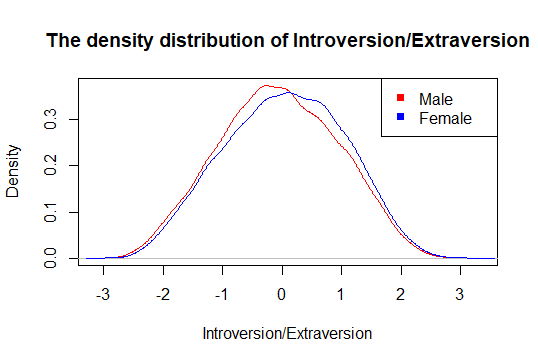
\includegraphics{Introversion_Extraversion.png}
  \caption{Introversion Extraversion.png}
  \end{center}
\end{figure}

{\normalsize{\bf the interpretation:}} \\\vspace{0.5cm}
the representation show that the graph is not symmetric allowing 
the mean wich equal 0.04  for the females and -0.06  for the males 

The result in this case that females are more Introversion/Extraversion than males



\begin{figure}[]
\setlength{\abovecaptionskip}{-4pt}
\begin{center}
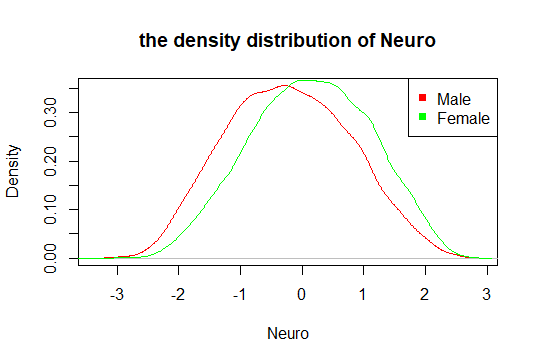
\includegraphics{Neuro.png}
  \caption{Neuro.png}
  \end{center}
\end{figure}
{\normalsize{\bf the interpretation:}} \\\vspace{0.5cm}
the representation show that the graph is not symmetric allowing 
the mean witch equal 0.14 for the females and -0.22 for the males 

The result in this case that females are more Neuro  than males


\begin{figure}[]
\setlength{\abovecaptionskip}{-4pt}
\begin{center}
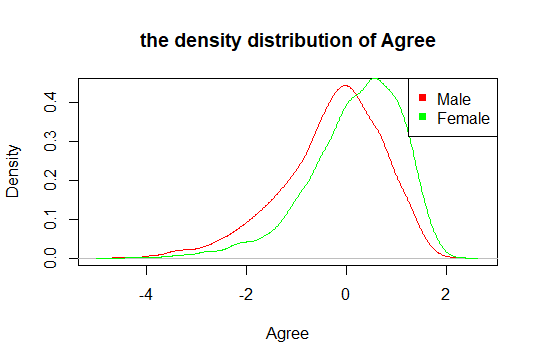
\includegraphics{Agree.png}
  \caption{Agree.png}
  \end{center}
\end{figure}
{\normalsize{\bf the interpretation:}} \\\vspace{0.5cm}
the representation show that the graph is not symmetric allowing 
the mean witch equal 0,18 for the females and -0.27 for the males
The result in this case that females are more Agree  than males

\begin{figure}[]
\setlength{\abovecaptionskip}{-4pt}
\begin{center}
  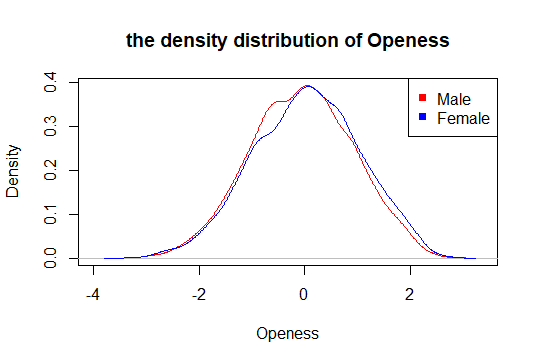
\includegraphics{openess.png} 
  \caption{openess.png}
\end{center}
\end{figure}
{\normalsize{\bf the interpretation:}} \\\vspace{0.5cm}
the representation show that the graph is not symmetric allowing 
the mean witch equal 0.036 for the females and -0.054 for the males
The result in this case that females are Openess than males

\begin{figure}[]
\setlength{\abovecaptionskip}{-4pt}
\begin{center}
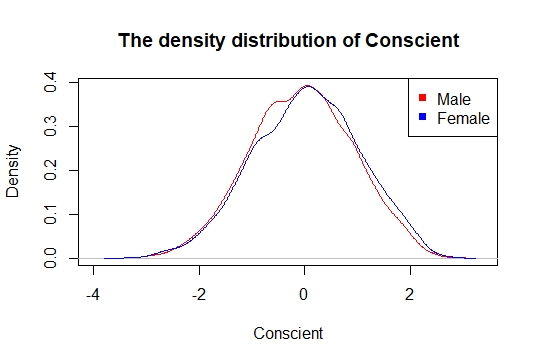
\includegraphics{Conscient.png}
  \caption{Conscient.png}
  \end{center}
\end{figure}

{\normalsize{\bf the interpretation:}} \\\vspace{0.5cm}
the representation show that the graph is not symmetric allowing 
the mean wich equal -0.092 for the females and 0.14 for the males
The result in this case that males are  more Consient  than females








\newpage
\section{Implementation/Simulation}
TODO: Show the implementation. The goal of this section is to show and explain the most important
parts of the code. Listing the code with highlighting and possibly line numbering is essential.
Explain the code by referring to line numbers, function calls and variable names.
Leave out trivial parts (initialization, parameter-tuning, etc...).
\newline
\underline{Data Preparation \href{https://github.com/Matthias2193/SPL/tree/master/Big5GritDataPreparation}{
\includegraphics[scale = 0.06]{Figures/qletlogo.pdf}} :} 
\newline 
This Quantlet translates data sets containing answers to a 50 item questionnaire into a data frame with the values of the personality traits according to the evaluation key. Optionally it can also deal with a data set from a questionnaire about grit. However, the data needs to contain the 50 items of the personality test. The order in which these answers are given does not matter since they are going to be reordered in the process of data cleaning.
\newline
The data "clean" function \href{https://https://github.com/Matthias2193/SPL/commit/7a9a8e8f543d93d635e4eeefad63280a26be99ad}{
\includegraphics[scale = 0.06]{Figures/qletlogo.pdf}Big5GritDataPreparation} takes the name of a data set, a boolean variable whether the data contains grit questionnaire and a survey date as parameters. This function can deal with excel data and data in the .csv format. It converts some of the numerical variable into factors and reorders the column. Before columns are converted the function checks whether they are null to prevent errors when trying to convert non existing columns. Unrealistic age values (greater than 100 or lower than 10) are also handled here. If a survey data is specified all age values larger than survey data - 101 are replaced by the absolute value of the survey date minus the age value. This approach is taken since a lot of people enter their birth year instead of their age. With this method we still get their actual age. For the remaining unrealistic age values a prediction model is build on the remaining variables and their age is predicted. The predicted at is rounded to the nearest integer. This approach lets us estimate a persons age so we are hopefully closer to the real value than if we just guessed or taken the mean/median. However, using a prediction model is prone to errors especially if used without specifying the input manually. Therefore, if there is an error during the prediction process the remaining unrealistic age values are replaced by random samples from the realistic ones. This way the guessed values resemble the distribution of the observed ones.
\newline
The "getResults" function \href{https://github.com/Matthias2193/SPL/blob/96a61ea2293d61c99c075877aca3accc1c847a22/Big5GritDataPreparation/Big5GritDataPreparation.R#L161-L195}{
\includegraphics[scale = 0.06]{Figures/qletlogo.pdf}Big5GritDataPreparation} transforms the questionnaire answers into the actual values of the personality traits and adds them to the data frame.
\newline
"getDataSetWithBig5" and "getGritDF" are the main methods that transform and return the Big 5 or Grit data set respectively. The columns of the returned data frames are always ordered with first the extra data (age, gender, nationality,...) then the 5 personality trait, and at the end Grit.
\newline
The "getCombinedData" function is basically a combination of the previous ones. This function only works if you have both Big 5 and Grit data and then combines them into one data frame omitting all columns that are only present in the latter. This method is used to combine our two data sets to give us more observations for analysis. It is however fairly specific to our case and will most likely not work properly with other data.
\newline
\newline
\underline{Data Preparation Analysis \href{https://github.com/Matthias2193/SPL/blob/master/SPL_Big5DataPreparationAnalysis/SPL_Big5DataPreparationAnalysis.R}{
\includegraphics[scale = 0.06]{Figures/qletlogo.pdf}} :} 
In this Quantlet we test how well principal component analysis and factor analysis estimate the scaled values obtained by using the evaluation key. Throughout this analysis the data worked with will often be just the answers to the questionnaires. To that end the columns will be selected using to numbers. 'Start' which is set to "which(colnames(data) == "E1")" and 'end' which is set to 'start + 49'. This is possible since the columns where sorted in this specific way during data cleaning.
\newline
The first step is estimating the correct number of pcs or factors to extract. This is done in several ways.
The first way is using the \href{https://www.rdocumentation.org/packages/psych/versions/1.8.4/topics/VSS}{vss} function implemented in R, which estimates the number of factors in a factor analysis. Another method is to do a parallel analysis to find both a good number for factors and pcs. The last method implemented is to do a simple PCA and to draw a screeplot. \href{https://github.com/Matthias2193/SPL/blob/3d1d23303132ad8092531f9474fbf78f5a8df3c5/SPL_Big5DataPreparationAnalysis/SPL_Big5DataPreparationAnalysis.R#L20-L54}{
\includegraphics[scale = 0.06]{Figures/qletlogo.pdf}SPL\_Big5DataPreparationAnalysis}.
\newline
In the code there are 3 functions implemented to extract the values via PCA as well as 1 function that uses factor analysis \href{https://github.com/Matthias2193/SPL/blob/3d1d23303132ad8092531f9474fbf78f5a8df3c5/SPL_Big5DataPreparationAnalysis/SPL_Big5DataPreparationAnalysis.R#L10-L16}{
\includegraphics[scale = 0.06]{Figures/qletlogo.pdf}SPL\_Big5DataPreparationAnalysis}. Those 4 functions all take a cleaned data frame as input and return a new data frame in which the questionnaire answers are replaced by the estimated values for the personality traits. Non-questionnaire columns remain unchanged. The functions for PCA differ in the PCA function they use. The 3 implemented are: \href{http://www.personality-project.org/r/html/principal.html}{principal}, \href{https://stat.ethz.ch/R-manual/R-devel/library/stats/html/prcomp.html}{prcomp} and \href{https://stat.ethz.ch/R-manual/R-devel/library/stats/html/princomp.html}{princomp}.  
\newline
Next the results of 'prcomp' and 'princomp' are compared in 2 ways. First, a screeplot is drawn for both results and then their centers and standard deviations are compared.
\newline
The main comparison of PCA, factor analysis and the evaluation key is done in two functions: 'compareDensities' and 'compareDifferences' \href{https://github.com/Matthias2193/SPL/blob/f6c320279a478642e8a87020ac48029a48624933/SPL_Big5DataPreparationAnalysis/SPL_Big5DataPreparationAnalysis.R#L78-L117}{
\includegraphics[scale = 0.06]{Figures/qletlogo.pdf}SPL\_Big5DataPreparationAnalysis}. Both function take the name of a data file as input. Then both transform the questionnaire answers to personality traits using the evaluation key, factor analysis and PCA ('princomp'). 'compareDensities' then uses a for loop to go through a vector with the names of the personality traits and draws a a plot containing the density distribution of all 3 methods for each personality trait.
\newline
'compareDifferences' simply compares the average difference between factor analysis and evaluation key vs. PCA and evaluation key.
\newline
In the data cleaning part it was mentioned that there is an option to combine 2 data set in order to have more observations. This is only possible if both data sets don't have overlap. Otherwise you would have the several observations twice in the combined data set. 
\newline
The last part of this analysis is a test to check for overlap between 2 datasets. To do this the 2 data sets are merged by the traits or by the remaining columns. The 'nrow' function then gives the number of matching pairs in the 2 data sets.  
\newline
\newline
\underline{Correlation Analysis \href{https://github.com/Matthias2193/SPL/blob/master/SPL_Big5CorrelationAnalysis/SPL_Big5CorrelationAnalysis.R}{
\includegraphics[scale = 0.06]{Figures/qletlogo.pdf}} :} 
\newline
This Quantlet shows the correlation first just between the five personality traits in a normal corrplot. Then it adds age and gender and displays the results in two mixed corrplots. Once unordered and once ordered by the angular order of the eigenvectors (AOE).
\newline
\underline{Cluster Analysis \href{https://github.com/Matthias2193/SPL/blob/master/SPL_Big5ClusterAnalysis/SPL_Big5ClusterAnalysis.R}{
\includegraphics[scale = 0.06]{Figures/qletlogo.pdf}} :} 
\newline
The goal of this Quantlet is to do some basic clustering on the personality traits plus age. First the data is clustered using k-Means with 2 to 5 clusters. Each time a plot is drawn displaying the results. To do this in a 2-dimensional space the dimensions are reduced using PCA during the plotting process. Additionally the mean values for the personality traits and age are printed out for each cluster after each clustering process. To do this 4 time a for-loop is used. \href{https://github.com/Matthias2193/SPL/blob/5c17336568167689696460c9166539babe69ee23/SPL_Big5ClusterAnalysis/SPL_Big5ClusterAnalysis.R#L10-L22}{
\includegraphics[scale = 0.06]{Figures/qletlogo.pdf}SPL\_Big5ClusterAnalysis}. This is done to give and initial overview over how different numbers of clusters will look and possibly provide an intuitive idea of the best number of clusters to actually use.
\newline
There are also 3 different tests implemented to estimate the best number of clusters to use. Those 3 methods are: 'Elbow methods', 'average silhouette' and 'GAP\_stat'. The 2 methods used for clustering are k-Means and 'partition around medoids' (PAM). Since clustering can be computing intensive the clustering is not done on the entire data set. Using the 'sample' function 2000 random elements of the dataset are selected for the analysis. For 'GAP\_stat' this number goes down to 1000, but the process might still take some time especially for (PAM). All of those test are run using the \href{https://www.rdocumentation.org/packages/factoextra/versions/1.0.5/topics/fviz_nbclust}{fviz\_nbclust} function.

\newpage
\section{Empirical Study/ Testing}


\ref{Fig:VSS}. 
\begin{figure}[ht]
    \begin{center}
        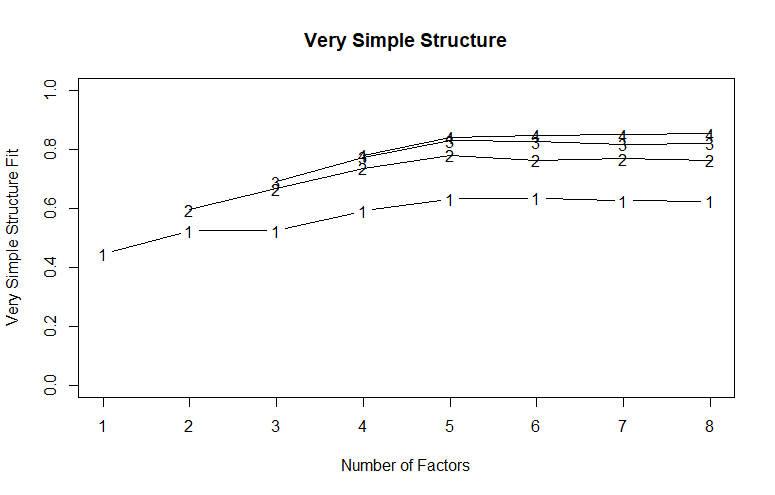
\includegraphics[scale=0.5,angle=0]{Figures/VSS.png}
        \caption{VSS-Analysis}
        \label{Fig:VSS}
    \end{center}
\end{figure}
\newline
The next method is to do a parallel analysis as seen in \ref{Fig:Parallel}.
\begin{figure}[ht]
    \begin{center}
        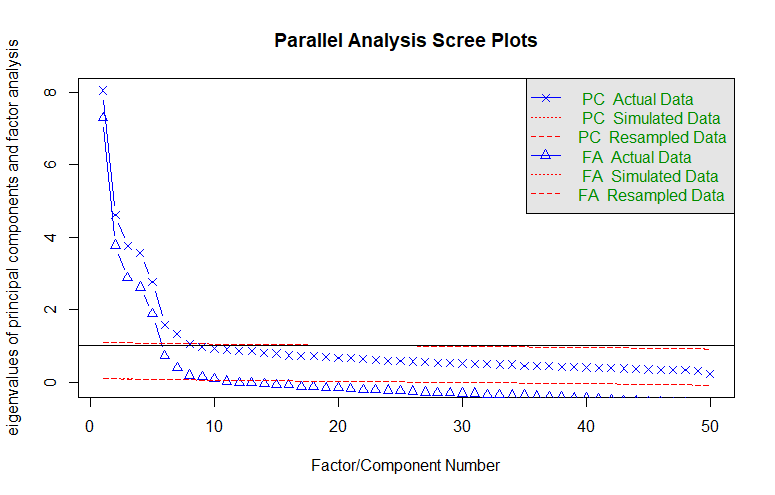
\includegraphics[scale=0.5,angle=0]{Figures/ParallelAnalysis.png}
        \caption{Parallel Analysis}
        \label{Fig:Parallel}
    \end{center}
\end{figure}
\newline

we tested our Data Analysis.R with P-value and T-student  to see whether it is significant or not  and then we compare  the mean of males and the mean of  females  to see which one of gender have thier special personality 

we concluded that in this table :

\begin{table}[ht]
    \begin{center}
        {\footnotesize
        \begin{tabular}{l|l|l|l|l|l|}
        \hline \hline
               & introversion   & neuro    & agree   & openess   & conscient        \\
            \hline
                Mean of males    & -0,06 & -0,22   & -0,27 & -0,054 & 0,14   \\
                Mean of females  & 0,04 & 0,14 & 0,18 & 0,036 & -0,092  \\
                t-student        & 7 & 25 & 31,5 & 6 & 16   \\
                p-value          & 1,213e-12 & 2,2e-16 & 2,2e-16 & 3,373e-10 & 2,2e-16   \\
               
            \hline \hline
        \end{tabular}}
    \end{center}
    
\end{table}

{\normalsize{\bf the results:}} \\\vspace{0.5cm}


we see that the t-student is bigger than T-table wich equal 1,65  with α=0,05     and  Degree of freedom (DF) is bigger than 29
  P-value is smaller than 0,05
and this confirm our rejection hypothesis that mean not equal to zero (or the mean of the females not equal the mean of males) 
  in case Introversion/Extraversion , Neuro, Agree and Openess
we see that the mean of the males is smaller than  the mean of  the females and that mean females are more Introversion/Extraversion,neuro, agree and openness than males
But in case Consient we see that the mean of the males is bigger than  the mean of  the females and that mean males are more consient than females 





TODO: Test your code with an empirical study. Describe the data you use, state the source and how
the data was prepared. Show tests of final code version. Tests may include correct input,
incorrect input, special cases and stress tests etc. Method of testing will vary with the
problem at hand. Present the empirical results of your analysis. Do the results support the
theory? If not, why? \underline{\textbf{This section is very important.}}
\newline
\newline
Display the tests with this format:
\begin{itemize}
  \item Input
  \item Expected output
  \item Actual output
  \item Comments
\end{itemize}


\underline{Data Analysis - Gender Groups:
 \href{https://github.com/Matthias2193/SPL/blob/master/Big5DataAnalysisAgeGender/DataAnalysis_PTGenderAgeGroup.R}{
\includegraphics[scale = 0.06]{Figures/qletlogo.pdf}} :} 
\newline 
\newline
 This file deals with an analysis of all five personality traits (Extraversion, Openness, Conscientiousness, Agreeableness, and Neuroticism) with accordance to the age group. In short, we analysed whether a personality trait changes on average over time. Note, that the analysis from this file was made for a visual interpretation. Among vast academic researches along the topic of personality research, Roberts et al. (2006) have devoted themselves to this specific subject indeed. They found out that an average change in personality traits across the life course appears.
 \newline \newline
 In our study we have tried to show such patterns as well. For that we wanted to receive a visual big picture of the personality traits across the life course with accordance to our data set. 
Our file, in which we applied this study, starts with the general data generation part. With the function source(), we are able to access another file or rather script in order to connect with the already prepared data set which we will need for this study. 
 \newline \newline
When we set up the connection to the main data script, we pulled the data to our script and declared the dataset from the function `getCombinedData(FALSE)' as fiveFactors. We set the last parameter of the function to `FALSE' as we do not want to scale our data output from the test result.
 \newline \newline 
For the next step we created three new data frames in accordance to continue with our study. With the apply function from the package “base” we are able to return a vector of the average personality traits for each age group obtained by applying the mean function on our matrix `fiveFactor' with accordance to their age category. In short we applied a condition in our mean calculation for the personality traits, which is the age category.
\newline \newline
As we already explained, please note that each age category represents 10 years. So, in other words, if the test person is 18 years old it will fall into the age category 2. Further the entry mean, refers to the statistic method to calculate the mean of the entries. The last entry `na.rm=T' simply means that the functions ignores NAs for their calculation.
\newline \newline
The vectors, which the `apply()' functions returned, were called `avgAge[1,9]', where [1,9] refers to each category eg. 1 has been named `avgAge1'.
The generated vectors have been bounded together to a data frame, which was named `ages'.  The function `rbind()' binds all vectors together and with the function “data.frame”, we are able to create a data frame. 
\newline \newline
The same procedure was also applied two more times, however, with an additional condition. The following two data frames, which we created should differ in gender. So, we did the same procedure, but only wanted to take into consideration either male (`fiveDactors\$gender ==1') or female (`fiveDactors\$gender ==2'). The additional condition was added by applying the logical AND `\&'.  
\newline \newline
The generated data frames with respect to the gender group, was defined as `mage' (mean of personality traits with accordance to the age category of the male test persons) and `fage' (same but with respect to only female test persons).
\newline \newline
For the visualisation of our data frames to detect possible changes in personalities across the life course, we continued with plotting the average personality traits with respect to the age group (combined all test persons, only males, and only females).
\newline \newline
In the following we will explain the code by the example of the personality trait `Extraversion'. The following personality traits were applied the exact same procedure, however, intuitively with accordance to the certain personality trait.
\newline \newline
With the function `plot()' we are able to plot our first vector. Our x-axis were assigned to the age categories (ageCat). We only took into consideration group 1-7, due to the fact that age group 8 and 9 showed massive deviation. For comparison, table (XC) will demonstrate it with the example of the personality trait `Extraversion'. The second entry of our `plot()' function referred to the specific personality trait with respect to all test persons (`ages\$Intro'). We selected the line type (our plotted vector should be shown as a line), we specified a colour and we scaled the y-axis for better visualisation. 
\newline \newline
To the generated plot for all test persons, we added two more lines (only males, only females). 
\newline \newline
\begin{figure}[ht]
\setlength{\abovecaptionskip}{-4pt}
\begin{center}
  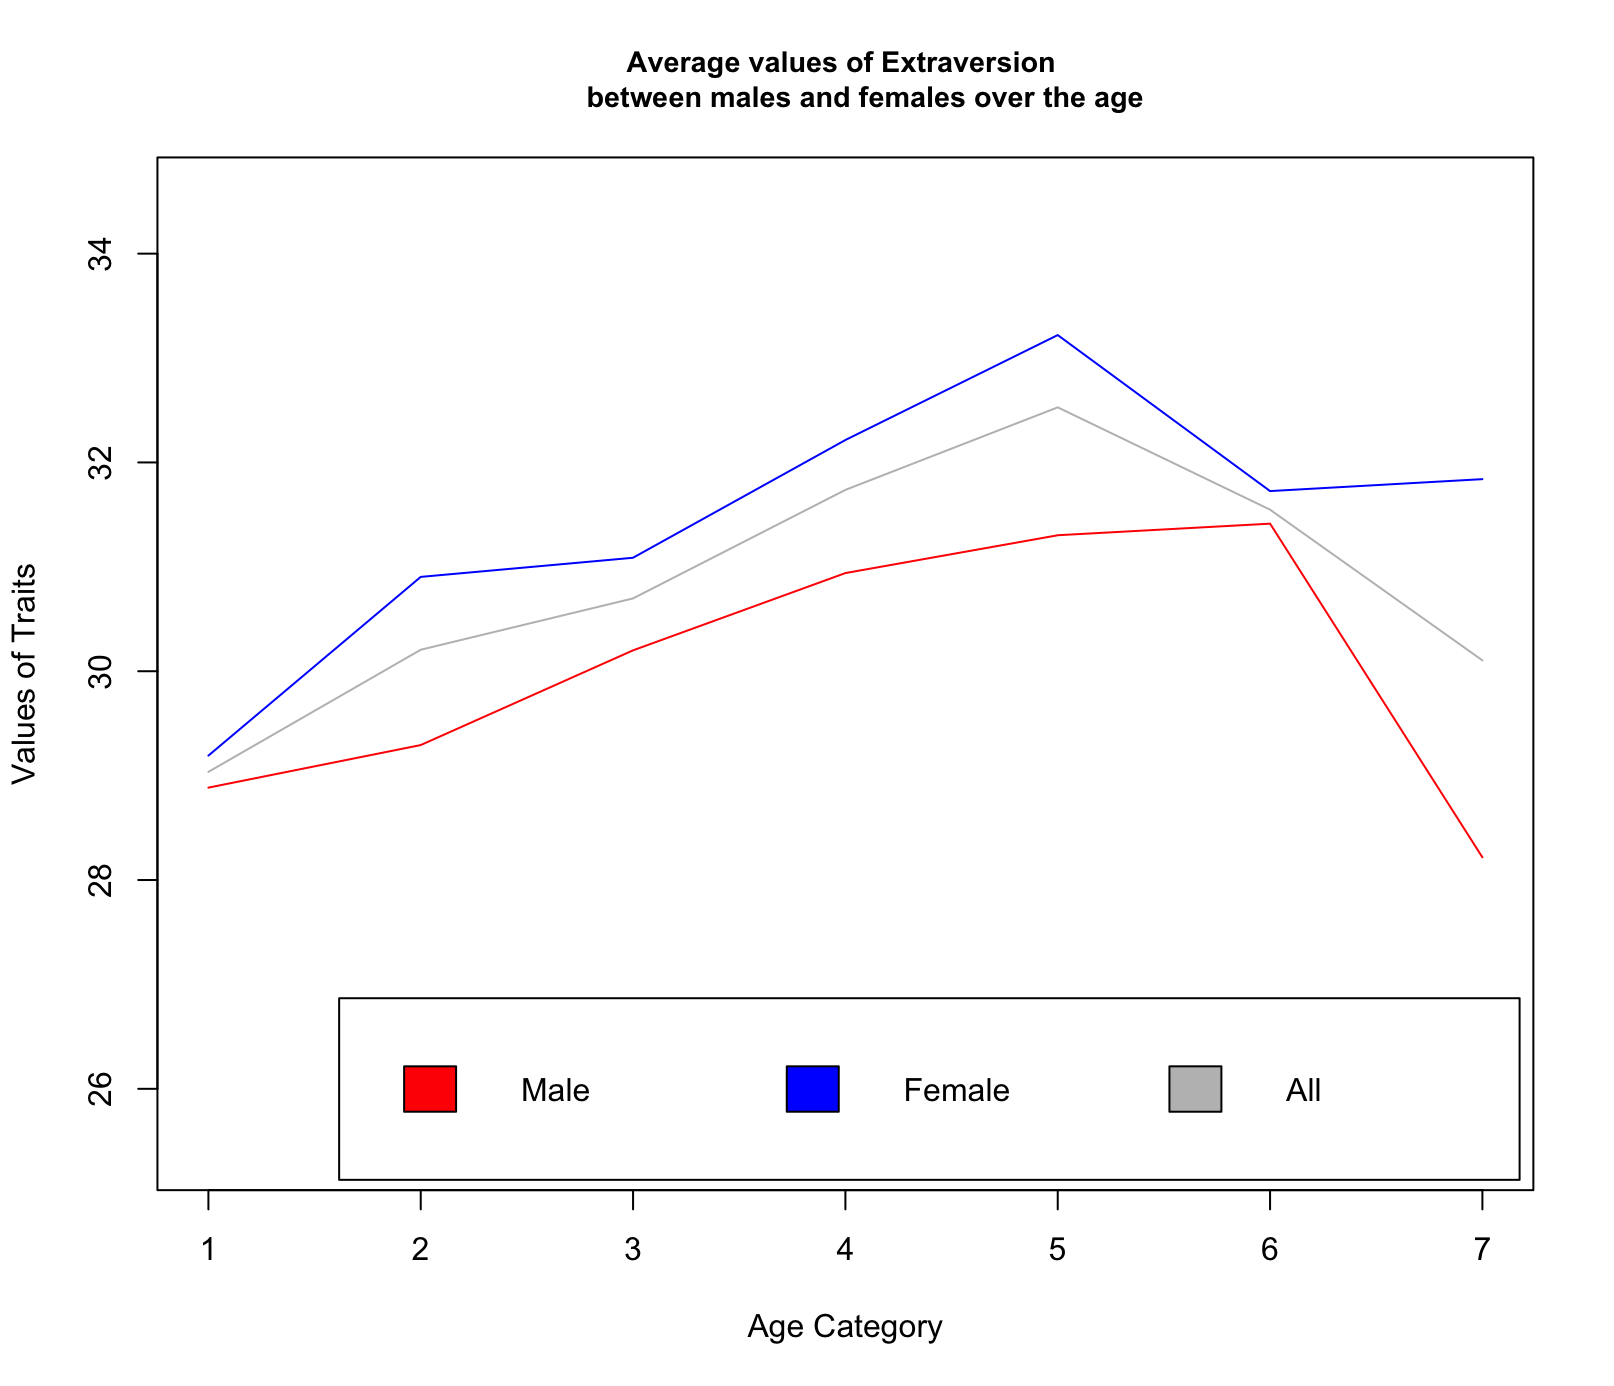
\includegraphics[width=13cm]{Figures/AVG_Extra_Gender}
  \caption{Personality Difference of Age and Gender}
\end{center}
\end{figure}
\newline \newline
With accordance to the figure above, we visually have similar findings as Roberts et al. (2006). Across the life course we have a changing value of trait. In other words, we can conclude that the average score of Extraversion (based on the test result) is increasing by age. However, in age category 5, we see a slightly decresing value for females. For men, we find that the personality (`Extraversion') is decreasing up from age group 6. 
\newline \newline
We have similar findings for our other personality traits. With accordance to our personality test data, we can visually conclude that across the life course we have a changing value. These findings are similar to these in Roberts et al. (2006).
\newline \newline
\underline{Data Analysis - Variance Analysis:
 \href{https://github.com/Matthias2193/SPL/tree/master/Big5VarianceAnalysis}{
\includegraphics[scale = 0.06]{Figures/qletlogo.pdf}} :} 
\newline 
\newline
Further with our study, in file `Variance Analysis – Big 5' we analysed the relationship between personality traits and age. As we have seen it visually that across the life course we have a changing value, we want to calculate that once working with regression models for our personality traits the additional variable age will significantly decrease the variance or rather the fit of the regression. The paper by Srivastava et al. (2003) studied whether the personality changes during adulthood. 
\newline \newline
Therefore, we tested our hypothesis from our visual results that age has an influence on the character over the course of life. 
\newline \newline
For that, we first applied an analysis of variance (ANOVA) in R. With the function `aov()' we were able to perform an ANOVA. We did our study first with the application whether the age of our test persons having a significant impact on the personality trait `Agreeableness'. Our ANOVA showed that the additional variable age improved the fit significantly (on all conventional significant levels). 
\newline \newline
Further, we created ANOVAs for all personality traits against the independent variable for age, hand, race and gender. Are these variables improving the fit and provide additional information?
\newline \newline
We created a function named \href{https://github.com/Matthias2193/SPL/blob/40438376a983799102d15acb98bdd9a0a98a6889/Big5VarianceAnalysis/VarianceAnalysis.R#L13-L26}{
\includegraphics[scale = 0.06]{Figures/qletlogo.pdf}anova\underline{ }multi} to solve this problem in accordance to receive a matrix with all our test results.
\newline \newline
The function first creates an empty matrix with the number of rows in accordance to the personality traits (we have 5) plus the number of columns in accordance to our independent variables (we have 4). The function `names()' calls the row names out of our dataset `DATA', in accordance to name the matrix with their row names. The column names were chosen based on the independent variable. We created a list for that: `c('Test Stat - Gender', 'Test Stat - Age', 'Test Stat - Hand', 'Test Stat - Race')'.
\newline \newline
With the for function we can calculate all the ANOVAs in an iterative way. It calculates for each column 5 times an ANOVA with the different personality traits, but the same independent variable. Once it’s done it will return the matrix in the console. 
\newline \newline
With this function, we are now able to create a matrix of the different p-values out of the F-statistic whether the independent variable increases the variance. A p-value smaller than 0.05 rejects the H0 (on a 5 \% significance level) that the independent variable does not increase fit of the regression. In other words, we want a rejection to conclude that the independent variable decreases the variance and therefore includes further information.
\newline \newline
With the function `anova\underline{ }multi(DATA,DATA{[,2]},DATA{[,3]},DATA{[,4]},DATA{[,5]})' we ran the function on our data set in accordance to the selected independent variables (gender, age, hand, race). 
\newline \newline
With respect to the table above, we can confirm that the personality changes across the course of life.
However, the independent variable `race' does not improve the fit for the personality Extraversion and Neuroticism. In other words, the variance for the regression, when considering “race” as an additional variable, does not decrease for these two. Conscientiousness is only decreasing the variance on a 10\% significant level. Overall, we can conclude that the ANOVA test is overall an important measurement for explaining the fact of personality traits with accordance to independent variables, in particular gender, age, hand, and race. When looking at the independent variables fundamentally, we support the fact for age as we refer to Srivastava et al. (2003). However, the other findings could overall not have a significant impact on explaining the personality traits. 



\newpage
\section{Conclusions}\label{Sec:Conc}

after this results we see that:


\begin{itemize}

    \item females are more Introversion/Extraversion,neuro, agree and openness than males

    \item males are more consient than females 
   
   \item Expose results concisely.

    \item Draw conclusions about the problem studied. What are the
    implications of your findings?

    \item Point out some limitations of study (assist reader in judging validity
    of findings).

    \item Suggest issues for future research.

\end{itemize}






% ----------------
% --- appendix ---
% ----------------
\appendix

% literature
\newpage
\addcontentsline{toc}{section}{References}
\bibliography{literature}

% figures (not mandatory)
\newpage
\section{Figures}

\begin{figure}[ht]
    \begin{center}
        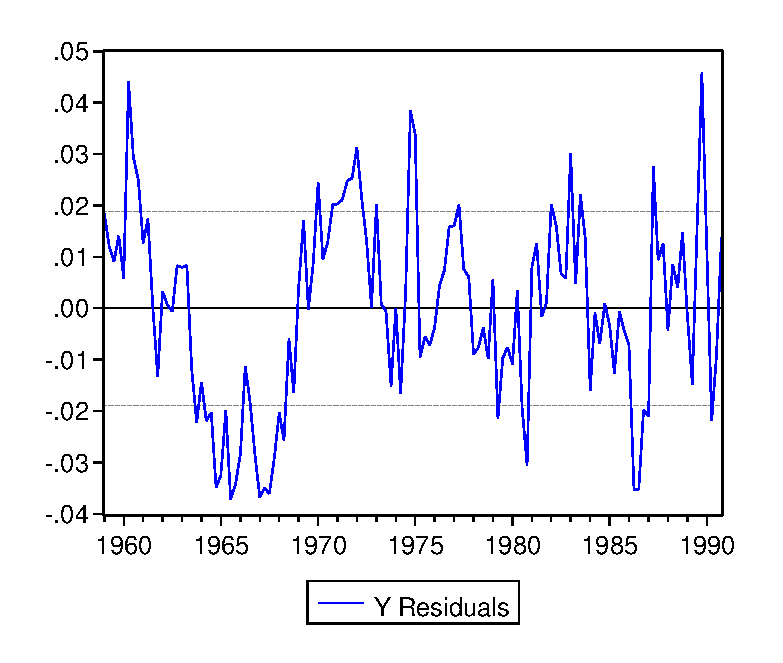
\includegraphics[scale=0.5,angle=0]{graph}
        \caption{Estimated residuals (2) from model XXX. ...}
        \label{Fig:Resids2}
    \end{center}
\end{figure}


% tables (not mandatory)
\newpage
\section{Tables}

\begin{table}[ht]
    \begin{center}
        {\footnotesize
        \begin{tabular}{l|l|l|l|l|l|}
        \hline \hline
               & introversion   & neuro    & agree   & openess   & conscient        \\
            \hline
                Mean of males    & -0,06 & -0,22   & -0,27 & -0,054 & 0,14   \\
                Mean of females  & 0,04 & 0,14 & 0,18 & 0,036 & -0,092  \\
                t-student        & 7 & 25 & 31,5 & 6 & 16   \\
                p-value          & 1,213e-12 & 2,2e-16 & 2,2e-16 & 3,373e-10 & 2,2e-16   \\
               
            \hline \hline
        \end{tabular}}
    \end{center}
    
\end{table}



% --------------------------------------------
% --- last page: Declaration of Authorship ---
% --------------------------------------------

\newpage
\thispagestyle{empty}
%{\Large{\bf Declaration of Authorship}}\vspace{0.5cm}

\section*{Declaration of Authorship}

We hereby confirm that we have authored this Seminar paper independently and without use
of others than the indicated sources. All passages which are literally or in general matter taken
out of publications or other sources are marked as such.
\vspace{1cm}

Berlin, September 30, 2007 \vspace{0.5cm}

your name (and signature, of course)



\end{document}
